%%%%%%%%%%%%%%%%%%%%%%%%%%%%%%%%%%%%%%%%%%%%%%%%%%%%%%%%%%%%%%%%%%%%
%% I, the copyright holder of this work, release this work into the
%% public domain. This applies worldwide. In some countries this may
%% not be legally possible; if so: I grant anyone the right to use
%% this work for any purpose, without any conditions, unless such
%% conditions are required by law.
%%%%%%%%%%%%%%%%%%%%%%%%%%%%%%%%%%%%%%%%%%%%%%%%%%%%%%%%%%%%%%%%%%%%

\documentclass{beamer}
\usetheme[faculty=phil]{fibeamer}
\usepackage[utf8]{inputenc}
\usepackage[
  main=english
]{babel}
%% These macros specify information about the presentation
\title{Classical Black Holes} %% that will be typeset on the
\subtitle{08. Accretion} %% title page.
\author{Edward Larra\~{n}aga}
%% These additional packages are used within the document:
\usepackage{ragged2e}  % `\justifying` text
\usepackage{booktabs}  % Tables
\usepackage{tabularx}
\usepackage{tikz}      % Diagrams
\usetikzlibrary{calc, shapes, backgrounds}
\usepackage{amsmath, amssymb}
\usepackage{url}       % `\url`s
\usepackage{listings}  % Code listings
\usepackage{siunitx}
\frenchspacing
\begin{document}
\frame{\maketitle}

\AtBeginSection[]{% Print an outline at the beginning of sections
\begin{frame}<beamer>
\frametitle{Outline for Part \thesection}
\tableofcontents[currentsection]
\end{frame}}

\section{Accretion Basics}
\begin{frame}
\Huge
Accretion Basics
\end{frame}

\begin{frame}{Accretion Basics}
	Process of matter falling into the potential well of a gravitating object.\\
\end{frame}

\begin{frame}{Accretion Regimes}
	\begin{enumerate}
	\item Spherical Accretion
	\item Cylindrical Accretion
	\item Accretion Disk
	\item Two-Stream Accretion 
	\end{enumerate}
\end{frame}

\begin{frame}{Spherical Accretion}
	\begin{itemize}
	\item No (significant) angular momentum
	\pause
	\item Determined by the relation between\\
	$c_s$: speed of sound in matter\\
	$v_{rel}$: relative velocity between accretor and matter
	\pause
	\item $v_{rel} \ll c_s$
	\pause	
	\item If the accretor is a BH, 
	$$v_{rel} = v$$
	$v$: velocity of accreting matter (i.e. the BH doesn't move!)  
	\end{itemize}
\end{frame}

\begin{frame}{Cylindrical Accretion}
	\begin{itemize}
	\item Small angular momentum
	\pause
	\item $v_{rel} \geq c_s$
	\end{itemize}
\end{frame}

\begin{frame}{Accretion Disk}
	\begin{itemize}
	\item Angular momentum is high enough to form an accretion disk
	\pause
	\item Matter spirals down into the accretor
	\end{itemize}
\end{frame}

\begin{frame}{Two-Stream Accretion}
	\begin{itemize}
	\item Quasi-spherically symmetric inflow coexist with an accretion disk
	\end{itemize}
\end{frame}

\subsection{Spherical Accretion}
\begin{frame}
	\huge
    Spherical Accretion
\end{frame}

\begin{frame}{Spherical Accretion}
	First model of accretion. Smooth and time-steady 	accretion.\\
	\pause
	\bigskip	
	We assume a completely ionized hydrogen gas cloud as the accretion structure.\\
	\pause
	\bigskip	
	Gas moves very slowly.  The description is made in terms of fluid mechanics equations.\\
	\pause
	\bigskip
	First and simplest description: To avoid the disintegration of the accretion structure, the outward force due to radiation pressure must be counterbalanced by the gravitational force.\\
\end{frame}

\begin{frame}{Radiation Pressure}
	Outward energy flux at distance $r$ from the center
	\[ F = \frac{L}{4\pi r^2}\]
	\pause
	$L$: bolometric luminosity [$\textrm{ erg} \cdot \textrm{s}^{-1}$]
	\pause
	For photons:
	\[ p^\mu = \left( \frac{E}{c}, \vec{p} \right) \qquad
	p^2 = \frac{E^2}{c^2} - |\vec{p}|^2 = 0\]
	\pause
	Then, the outwards momentum flux (or pressure) is
	\[P_{rad} = \frac{F}{c} = \frac{L}{4\pi r^2 c}\] 
\end{frame}

\begin{frame}{Radiation Pressure}
	The radiation force on a single electron is
	\[\vec{f}_{rad} = ( \sigma_e P_{rad} ) \hat{r} = \sigma_e \frac{L}{4\pi r^2 c} \hat{r}\] 
	\pause
	$\sigma_e$: Thomson cross-section
	\pause
	\[\sigma_e = \frac{8\pi}{3} \left( \frac{e^2}{m_e c^2} \right)^2 = 6.65 \times 10^{-25} \textrm{ cm}^2 \]
	\footnotesize
	Interaction with protons is negligible because it is lower by a factor of $\left(\frac{m_p}{m_e}\right)^2 \sim 3 \times 10^6$
\end{frame}

\begin{frame}{Gravitational Force}
	The gravitational force between the central object $M$ and one electron-proton pair is
	\pause
	\[\vec{f}_g = -\frac{GM(m_e + m_p)}{r^2} \hat{r} \sim -\frac{GM m_p}{r^2} \hat{r}\]
\end{frame}

\begin{frame}{Spherical Accretion}
	To avoid the disintegration of the accretion structure,
	\pause
	\[|\vec{f}_{rad}| \leq | \vec{f}_g|\]
	\pause
	\[ \sigma_e \frac{L}{4\pi r^2 c} \leq \frac{GM m_p}{r^2} \]
	\pause
	\[ L \leq \frac{4 \pi GM m_p c}{\sigma_e} \]
\end{frame}

\subsection{Eddington Luminosity}
\begin{frame}{Eddington Luminosity}
	\[ L \leq L_E \]
	\pause
	\[ L_E = \frac{4 \pi GM m_p c}{\sigma_e} \]
	\pause
	\[ L_E = 6.31 \times 10^4 M \textrm{ [erg} \cdot \textrm{s}^{-1} \cdot \textrm{kg}^{-1} \textrm{]}  \]
	\pause
	\[ L_E = 1.26 \times 10^{38} \left(\frac{M}{M_\odot\ } \right) \left[ \textrm{ erg} \cdot \textrm{s}^{-1} \right] \]
	\pause
	\footnotesize
	Eddington Lumionisty: Maximum luminosity of a source $M$ powered by spherical accretion.
\end{frame}

\subsection{Estimation of the Central Mass}
\begin{frame}{Estimation of the Central Mass from its Luminosity}
	\[ M \geq \frac{L \sigma_e}{4 \pi G m_p c} \]
	\pause
	\[ M \geq \frac{L}{1.26 \times 10^{38}} \left[ M_{\odot\ } \right] \]
	\pause
	\[ M \geq 8 \times 10^5 L_{44} \left[ M_{\odot\ } \right] \]
	\pause
	\footnotesize
	$L_{44}$: Central Source Luminosity in units of $10^{44} \textrm{ erg} \cdot \textrm{s}^{-1}$ (typical value for AGN's)\\
	\pause
	
	$M_E = 8 \times 10^5 L_{44} M_{\odot\ }$: \textit{Eddington's Mass}. Minimum mass for a given luminosity
\end{frame}

\begin{frame}{Estimation of the Central Mass from its Luminosity}
	AGN's have typically $L \sim 10^{43} - 10^{47} \textrm{ erg} \cdot \textrm{s}^{-1}$\\	
	\pause
	
	Black holes with $ M \sim 10^5 - 10^9 M_{\odot\ }$
\end{frame}

\begin{frame}{Estimation of the Central Mass from its Luminosity}
	\begin{center}
      \begin{figure}
      	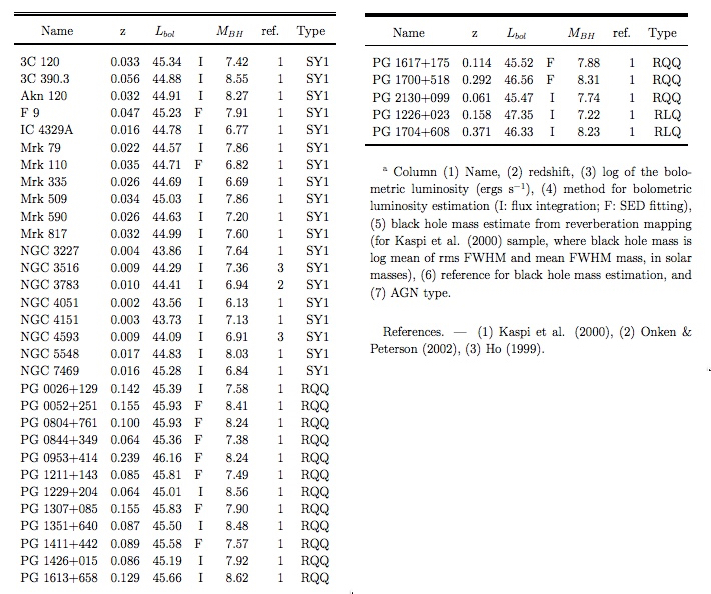
\includegraphics[scale=0.3] {figures/AGNs.jpg}
      \end{figure}
	\end{center}	
	\tiny
	J.-H. Woo, C. M. Urry. \textit{AGN Black Hole Masses and Bolometric Luminosities}. \textit{Astrophys. J.} 579 (2002) 530-544
\end{frame}

\subsection{Eddington Accretion Rate}
\begin{frame}{ Accretion Rate}
	The luminosity is just a fraction of the relativistic energy of the accreting mass, $E=m c^2$. The other fraction goes into the BH making it grow.
	\pause
	\[ L \propto \frac{dE}{dt} = \frac{dm}{dt} c^2 = \frac{dM}{dt} c^2 \]
	\pause
	\[L = \eta \dot{M} c^2\]
	\pause
	$\eta$: Efficiency of the process
\end{frame}


\begin{frame}{ Accretion Rate}
	Accretion produces radiation by conversion of gravitational potential.
	\[ U = \frac{GMm}{r}\]
	\pause
	\[ L \sim \frac{dU}{dt} = \frac{GM}{r} \frac{dm}{dt} = \frac{GM}{r} \dot{M} \]
	\pause
	\[\eta = \frac{GM}{rc^2}	\]	
\end{frame}

\begin{frame}{ Accretion Rate}
	In order to estimate the efficiency, consider the ISCO for Schwarzchild, 
	\[r_{ISCO} = 3r_S = \frac{6GM}{c^2}\]
	\pause
	A particle falling from this orbit into the BH  looses the energy
	\pause
	Hence
	\pause
	\[\eta \sim 0.1 - 0.2 \]	
\end{frame}

\begin{frame}{ Accretion Rate}
	In some books consider the accretion of particles falling from $r=5r_S$, because it gives most of the optical/UV continuum radiation.\\
	\pause
	
	Using this point, one obtains an efficiency of $\eta \sim 0.1$
\end{frame}

\begin{frame}{ Accretion Rate}
	For a typical AGN, $L \sim 10^{47} \textrm{ erg} \cdot \textrm{s}^{-1}$.\\
	\pause
	\begin{itemize}
	\item If $\eta \sim 0.007$ as in the Hydrogen burning process (Nuclear fusion), it gives
	\pause
	\[\dot{M} = \frac{L}{\eta c^2} \sim 250 M_{\odot\ } \cdot \textrm{yr}^{-1} \]
	\pause
	\item If $\eta \sim 0.1 $ we obtain a more realistic value of
	\pause
	\[\dot{M} = \frac{L}{\eta c^2} \sim 250 M_{\odot\ } \cdot \textrm{yr}^{-1} \]
	\pause
	\end{itemize}		
\end{frame}

\begin{frame}{ Accretion Rate}
	\[ \dot{M} = \frac{L}{\eta c^2} = 1.11 \times 10^{23} \frac{L_{44}}{\eta} \left[ \frac{\textrm{gr}}{\textrm{s}}\right]\]	
	\pause
	\[ \dot{M} = 1.77 \times 10^{-2} L_{44} \left ( \frac{\eta}{0.1}\right)^{-1} \left[ \frac{M_{\odot\ }}{\textrm{yr}}\right]\]
\end{frame}

\begin{frame}{Eddington Accretion Rate}
	\[ \dot{M}_E = \frac{L_E}{\eta c^2} =  \frac{4 \pi GM m_p}{\sigma_e \eta c} \]	
	\pause
	\[ \dot{M}_E = 2.67 \times 10^{-8} \left ( \frac{\eta}{0.1}\right)^{-1} \frac{M}{M_{\odot\ } }  \left[ \frac{M_{\odot\ }}{\textrm{yr}}\right]\]
	\pause
	\[ \dot{M}_E = 3 \left ( \frac{\eta}{0.1}\right)^{-1} M_8   \left[ \frac{M_{\odot\ }}{\textrm{yr}}\right]\]
	\pause
	$\dot{M}_E$: Maximum possible accretion rate for a mass $M_8 = \frac{M}{10^8 M_{\odot\ }}$.
\end{frame}

\begin{frame}{Eddington Accretion Rate}
	May $\dot{M} > \dot{M}_E$ ?
	\pause
	\begin{enumerate}
		\item It depends on a careful determination of $\eta$. E.g. if $\eta < 0.1$, the outwards flux is diminished.
		\pause
		\item $\dot{M}_E$ can be exceeded with non-spherical models.
	\end{enumerate}
\end{frame}

\subsection{Growth Time}
\begin{frame}{Growth Time}
	\[ \dot{M} = \frac{dM}{dt} = \frac{L}{\eta c^2} \]
	\pause
	\[ \dot{M} = \frac{dM}{dt} = \frac{L}{L_E} \frac{4 \pi GM m_p}{\sigma_e \eta c} \]
	\pause
	\[ \int \frac{dM}{M} = \frac{L}{L_E} \frac{4 \pi G m_p}{\sigma_e \eta c} \int dt \]
	\pause
	\[ M(t) = M_0 \exp \left( \frac{t}{t_{growth} }\right) \]
	\pause
	\[ t_{growth} = \frac{\sigma_e \eta c}{4 \pi G m_p} \left( \frac{L_E}{L} \right) \]
\end{frame}

\begin{frame}{Growth Time}
	\[ t_{growth} = \frac{\sigma_e \eta c}{4 \pi G m_p} \left( \frac{L_E}{L} \right) \]
	\pause
	\[ t_{growth} = 3.7 \times 10^8 \eta \left( \frac{L_E}{L} \right) [\textrm{yr}]\]
	\pause
	\footnotesize
	For $L \sim L_E$, the BH grows exponentially on time scales of the order $\sim 10^8 \textrm{ yr}$.
\end{frame}

\subsection{Temperatures}
\begin{frame}{Radiation Temperature}
	The \textit{continuum spectrum} of the emitted radiation is characterized by a temperature
	\[ T_{rad} = \frac{h\bar{\nu}}{k_B}\]
	\pause	
	$\bar{\nu}$: frequency of a typical (average) photon
\end{frame}

\begin{frame}{Black Body Temperature}
	For a source with accretion luminosity $L$ and radius $r$, it is defined the \textit{blackbody temperature} through
	\[F= \sigma T_{eff}^4 \]
	\pause	
	$\sigma = 5.6 \times 10^{-5} \frac{\textrm{erg}}{\textrm{cm}^2 \cdot \textrm{s} \cdot \textrm{K}^4 \cdot \textrm{sr}}$\\
	Steffan-Boltzman Constant
	\pause
	\[ T_{eff} = \left( \frac{L}{4\pi r^2 \sigma} \right)^{1/4} \]
\end{frame}

\begin{frame}{Black Body Temperature}	
	Using $L = \frac{GM}{r} \dot{M}$,
	\pause	
	\[ T_{eff} = \left( \frac{GM\dot{M}}{4\pi r^3 \sigma} \right)^{1/4} \]
	\pause
	\[T_{eff} = 1.01 \times 10^6 M_8^{-1/4} \left( \frac{\dot{M}}{\dot{M}_E} \right)^{1/4} \left( \frac{r}{r_S} \right)^{-3/4} \]
\end{frame}

\subsection{Compactness}
\begin{frame}{compactness}	
	One way to estimate the compactness of a source is using the luminosity and the effective surface temperature.
	\[r_{BB} = \sqrt{\frac{L}{4\pi \sigma T_{eff} ^4}}  \]
\end{frame}


\begin{frame}{Example}	
	Consider a system in our galaxy with $L=10^{37} \textrm{ erg} \cdot \textrm{s}^{-1}$
	\pause
	\bigskip
	From the Eddington limit, the mass of the central object must be
	\[ M \geq \frac{L}{1.26 \times 10^{38}} M_{\odot\ } \sim \frac{10^{37}}{10^{38}} M_{\odot\ }  \sim 0.1 M_{\odot\ } \]
\end{frame}

\begin{frame}{Example}	
	If the radiation is in the optical-UV,\\
	\onslide<2->
	
	$\nu_{max} \sim 10^{15} \textrm{Hz}$
	\onslide<3->
	\[ T_{eff} \sim T_c = \frac{10^{15}}{5.88 \times 10^{10}} \sim 10^5 \textrm{K} \]
	\onslide<4->
	\[ r_{bb} \sim 10^{12} \textrm{cm} \sim 10^{7} \textrm{km}\]
	\onslide<5->
	Typical size of a Star!
	
	\onslide<1->
	\tiny
	https://rechneronline.de/spectrum
\end{frame}

\begin{frame}{Example}	
	If the radiation is in soft X-rays at $1 \textrm{ keV}$,\\
	\onslide<2->
	
	$\nu_{max} \sim 10^{17} \textrm{Hz}$
	\onslide<3->
	\[ T_{eff} \sim T_c = \frac{10^{17}}{5.88 \times 10^{10}} \sim 10^7 \textrm{K} \]
	\onslide<4->
	\[ r_{bb} \sim 10^{6} \textrm{cm} \sim 10 \textrm{km}\]
	\onslide<5->
	Typical size of a neutron star or a BH!
	\onslide<1->
	\tiny
	https://rechneronline.de/spectrum
\end{frame}

\begin{frame}{Virial Temperature}	
	$T_{th}$: Temperature reached by the accreted material if all the gravitational energy is transformed into thermal energy.\\
	\pause
	$2\left\langle K \right\rangle + \left\langle U \right\rangle = 0$: Virial Theorem
	\pause
	\[ \left\langle U \right\rangle = \frac{GM(m_p + m_e)}{r}\sim \frac{GMm_p}{r} \]
	\pause
	\[ 2\left\langle K \right\rangle \sim 2 \times \frac{3}{2} k_B T_{th} \]
	\pause
	\[ T_{th} = \frac{GMm_p}{3k_B r} = T_{vir}\]
\end{frame}

\begin{frame}{Temperatures}	
	If the accretion energy is converted directly into radiation escaping without interaction,
	\pause
	\[ T_{rad} \sim T_{th}\]
	\pause
	If the accretion flow is optically thick, the radiation reaches thermal equilibrium with the accreted material before escaping out to the observer,
	\pause
	\[ T_{rad} \sim T_{eff}\]
	\pause
	\bigskip
	In general,
	\pause
	\[ T_{eff} \lesssim T_{rad} \lesssim T_{th}\]
	
\end{frame}



\section{Hydrodynamics Description of Spherical Accretion}    
\begin{darkframes}

\begin{frame}
\Huge
Hydrodynamics Description of Spherical Accretion
\end{frame}

\begin{frame}{Hydrodynamics Description of Spherical Accretion}
	Assumptions:
	\pause
	\begin{itemize}
	\item No viscosity
	\pause
	\item No angular momentum
	\pause
	\item No electromagnetic fields
	\end{itemize}	
	We are looking for
	\pause
	\begin{itemize}
	\item Steady accretion rate $\dot{M}$ in terms of the asymptotic density and temperature of the gas, $\rho_\infty$ and $T_\infty$.
	\pause
	\item Size of region where gas is influenced by the gravity of the BH
	\pause 
	\item Local velocity of the gas and local speed of sound
	\pause
	\item Spectrum of the emitted radiation by the accretion structure
	\end{itemize}
\end{frame}

\subsection{Hydrodynamics Equations}
\begin{frame}
\Huge
Hydrodynamics Equations
\end{frame}

\begin{frame}{Hydrodynamics Equations}
    \[ \frac{\partial \rho}{\partial t} + \vec{\nabla} \cdot \left( \rho \vec{v}\right) = 0 \]
    \center{Continuity Equation}
    \pause
    \bigskip
    \justify
	$\rho$: Mass density\\
	$\vec{v}$: Velocity of the gas
\end{frame}

\begin{frame}{Hydrodynamics Equations}
	\[ \rho \left[\frac{\partial \vec{v}}{\partial t} + \left( \vec{v} \cdot \vec{\nabla} \right) \vec{v} \right]
	= -\vec{\nabla} P + \rho \vec{g} + \vec{\nabla} \cdot \vec{\sigma}\]
	\center{Conservation of Momentum (ignoring radiation pressure)} 
	\pause
	\bigskip
	\justify
	$P$: Pressure\\
	$\vec{g}$: Acceleration due to gravity\\
	\pause  
	If self-gravity of the accretion structure is negligible,
	\[ \vec{g} = -\vec{\nabla} \Phi = -\frac{GM}{r^2} \hat{r}\]
\end{frame}

\begin{frame}{Hydrodynamics Equations}
	\[ \rho \left[\frac{\partial \vec{v}}{\partial t} + \left( \vec{v} \cdot \vec{\nabla} \right) \vec{v} \right]
	= -\vec{\nabla} P + \rho \vec{g} + \vec{\nabla} \cdot \vec{\sigma}\]
	\center{Conservation of Momentum (ignoring radiation pressure)} 
	\pause
	\bigskip
	\justify
	$\sigma_{ij}$: Viscosity Stress Tensor 
	\pause
	\[ \sigma_{ij} = 2\eta \tau_{ij} \]
	\pause
	\[ \tau_{ij} = \frac{1}{2} \left( \frac{\partial v_i}{\partial x^j} + \frac{\partial v_j}{\partial x^i}
	- \frac{2}{3} \frac{\partial v_k}{\partial x^k} \delta_{ij} \right)\]
\end{frame}

\begin{frame}{Hydrodynamics Equations}
	\[ \rho \left[\frac{\partial \vec{v}}{\partial t} + \left( \vec{v} \cdot \vec{\nabla} \right) \vec{v} \right]
	= -\vec{\nabla} P + \rho \vec{g} + \vec{\nabla} \cdot \vec{\sigma}\]
	\center{Conservation of Momentum (ignoring radiation pressure)} 
	\pause
	\bigskip
	\justify
	\[ \sigma_{ij} = 2\eta \tau_{ij} \]
	\pause
	\[ \eta = \rho \nu\]
	\pause
	$\eta$: dynamic viscosity\\
	$\nu$: kinematic viscosity\\
	
	\pause
	(we will assume $\nu = 0 $ for spherical accretion!)\\
	\pause
	\tiny
	* No-viscosity: Euler equation\\
	* Viscosity: Navier-Stokes equation
\end{frame}

\begin{frame}{Hydrodynamics Equations}
	\[ P = P(\rho) \]
	\center{Equation of state} 
	\pause
	\bigskip
	\justify
	Usually a polytropic: $P \propto \rho^\gamma $\\
	\pause
	\bigskip
	$1\leq \gamma \leq \frac{5}{3}$\\
	
	$\gamma = 1$: Iosthermic flow\\
	
	$\gamma = \frac{5}{3}$: Adiabatic flow
\end{frame}

\begin{frame}{Hydrodynamics Equations}
	\[ \rho \frac{d \varepsilon}{dt} = -P \vec{\nabla}\cdot \vec{v} 
	+ 2\eta \left[ S_{ij} S_{ij} - \frac{1}{3} (\vec{\nabla}\cdot \vec{v})^2 \right] + Q \]
	\center{Energy Balance} 
	\pause
	\bigskip
	\justify
	$\varepsilon$: Internal energy per unit mass of the fluid\\
	\pause
	$Q$: Net heat exchanged by an element of the fluid per unit time per unit volume\\
	\pause
	\[S_{ij} = \tau_{ij} - \frac{1}{3} (\vec{\nabla}\cdot \vec{v})\delta_{ij} \]
\end{frame}

\begin{frame}{Hydrodynamics Equations}
	\[ T = 	\frac{\mu m_H}{k_B} \frac{P}{\rho} \]
	\center{Perfect gas temperature} 
	\pause
	\bigskip
	\justify
	$m_H \sim m_p$: Hydrogen mass\\
	\bigskip
	\pause
	$\mu$: Mean molecular weight\\
	$\mu = 1$ for neutral Hydrogen\\
	$\mu = \frac{1}{2}$ for fully ionized Hydrogen
\end{frame}


\subsection{Spherical Accretion Hydrodynamics}
\begin{frame}
	\huge
    {Spherical Accretion Hydrodynamics}
\end{frame}

\begin{frame}{Spherical Accretion Hydrodynamics}
    Spherical symmetry and steady state:
    \pause
    \[ \rho = \rho(r) \]
    \[ \vec{v} = v(r) \hat{r}\]
\end{frame}

\begin{frame}{Continuity Equation}
    \[ \frac{\partial \rho}{\partial t} + \vec{\nabla} \cdot \left( \rho \vec{v}\right) = 0 \]
    \pause
    \[ \frac{1}{r^2} \frac{\partial}{\partial r} \left( r^2 \rho v \right) = 0\]
    \pause
    Integrating,
    \pause
    \[ \dot{M} = 4\pi r^2 \rho v \]
\end{frame}

\begin{frame}{Conservation of Momentum}
    \[ \rho \left[\frac{\partial \vec{v}}{\partial t} + \left( \vec{v} \cdot \vec{\nabla} \right) \vec{v} \right]
	= -\vec{\nabla} P + \rho \vec{g} \]
    \pause
    \[ v \frac{dv}{dr} + \frac{1}{\rho} \frac{\partial P}{\partial r} + \frac{GM}{r^2} = 0\]
\end{frame}

\begin{frame}{Equations Governing Spherical Accretion}
	\begin{align*}
	\dot{M} = 4\pi r^2 \rho v & \\
	v \frac{dv}{dr} + \frac{1}{\rho} \frac{\partial P}{\partial r} + \frac{GM}{r^2} &= 0 \\
	P \propto \rho^\gamma &
	\end{align*}	    
\end{frame}

\begin{frame}{Local Speed of Sound}
	\[ c_s ^2 = \gamma \frac{P}{\rho} \]	 
	\pause
	Sonic radius: The gas moves with the speed of sound,
	\[ r_s = \frac{GM}{2c_s^2}\]   
\end{frame}

\begin{frame}{Behavior of the gas in the accretion structure}
	For $r \gg r_s$
	\pause
	\begin{align*}
	c_s & \approx c_\infty \left[ 1- \frac{\gamma -1}{4} \frac{r_{acc}}{r}\right] \approx c_\infty\\
	v & \approx \frac{c_\infty}{16} \left( \frac{2}{5-3\gamma}\right)^{\frac{5-3\gamma}{2(\gamma-1)}}
	\left( \frac{r_{acc}}{r}\right)^2 \left[ 1- \frac{1}{2} \frac{r_{acc}}{r} \right] \approx 0\\
	\rho & \approx \rho_\infty \left[ 1- \frac{1}{2} \frac{r_{acc}}{r} \right] \approx \rho_\infty
	 \end{align*}
	 \pause	 
	$r_{acc} = \frac{2GM}{c_\infty^2} $: Accretion radius 
\end{frame}

\begin{frame}{Behavior of the gas in the accretion structure}
	For $r \ll r_s$
	\pause
	\begin{align*}
	v & \approx \sqrt{\frac{2GM}{r}} = v_{ff} \\
	\rho & \approx \rho (r_s) \left( \frac{r_s}{r}\right)^\frac{3}{2}
	 \end{align*}
\end{frame}

\begin{frame}{Temperature of the gas in the accretion structure}
	\[ T = 	\frac{\mu m_H}{k_B} \frac{P}{\rho} \]
	\pause
	\[ T = T(r_s) \left( \frac{r_s}{r}\right)^{\frac{3}{2}(\gamma - 1)} \]
\end{frame}

\begin{frame}{Temperature of the gas in the accretion structure}
	First law of thermodynamics:
	\[ d\varepsilon = dQ - PdV\]
	\pause
	\[ d\varepsilon = dQ + \frac{k_B}{\mu m_H} \frac{T}{\rho} d\rho\]	
	\pause
	Bremsstrahlung (free-free) radiation\\
	\pause
	$\frac{dQ}{dt} = -\alpha_{ff} T^{1/2} \rho$\\
	\pause
	$\alpha_{ff} \approx 5 \times 10^{20} \textrm{ erg} \textrm{ cm}^3 \textrm{ g}^{-2} \textrm{ s}^{-1} \textrm{ K}^{-1/2}$ for Hydrogen.	
\end{frame}

\begin{frame}{Temperature of the gas in the accretion structure}
	\[ \frac{dT}{dr} = - \frac{T}{r} - \alpha_{ff} \rho(r_s) \sqrt{\frac{r_s}{2GM}} \frac{T^{1/2}}{r} 
	\left( \frac{2\mu m_H}{3k_B} r_s\right) + \frac{2\mu m_H}{3k_B} \frac{dQ}{dr} \]
\end{frame}

\begin{frame}{Temperature of the gas in the accretion structure}
	If there is only Bremsstrahlung radiation, 	
	\[ \frac{dT}{dr} = - \frac{T}{r} - \alpha_{ff} \rho(r_s) \sqrt{\frac{r_s}{2GM}} \frac{T^{1/2}}{r} 
	\left( \frac{2\mu m_H}{3k_B} r_s\right) \]
	\pause
	Therefore,
	\[ \frac{dT}{dr}<0\]
	\pause
	The temperature of the flow decreases as the gas approaches the BH (\textit{cooling flow}).
\end{frame}

\begin{frame}{Temperature of the gas in the accretion structure}
	\[T = \left[ -\frac{4}{K} + \sqrt{\frac{16}{K^2} + \frac{4}{K\sqrt{r}} +C}\right]^2 \]
\end{frame}

\end{darkframes}
\begin{frame}{Temperature of the gas in the accretion structure}
	\begin{center}
      \begin{figure}
      	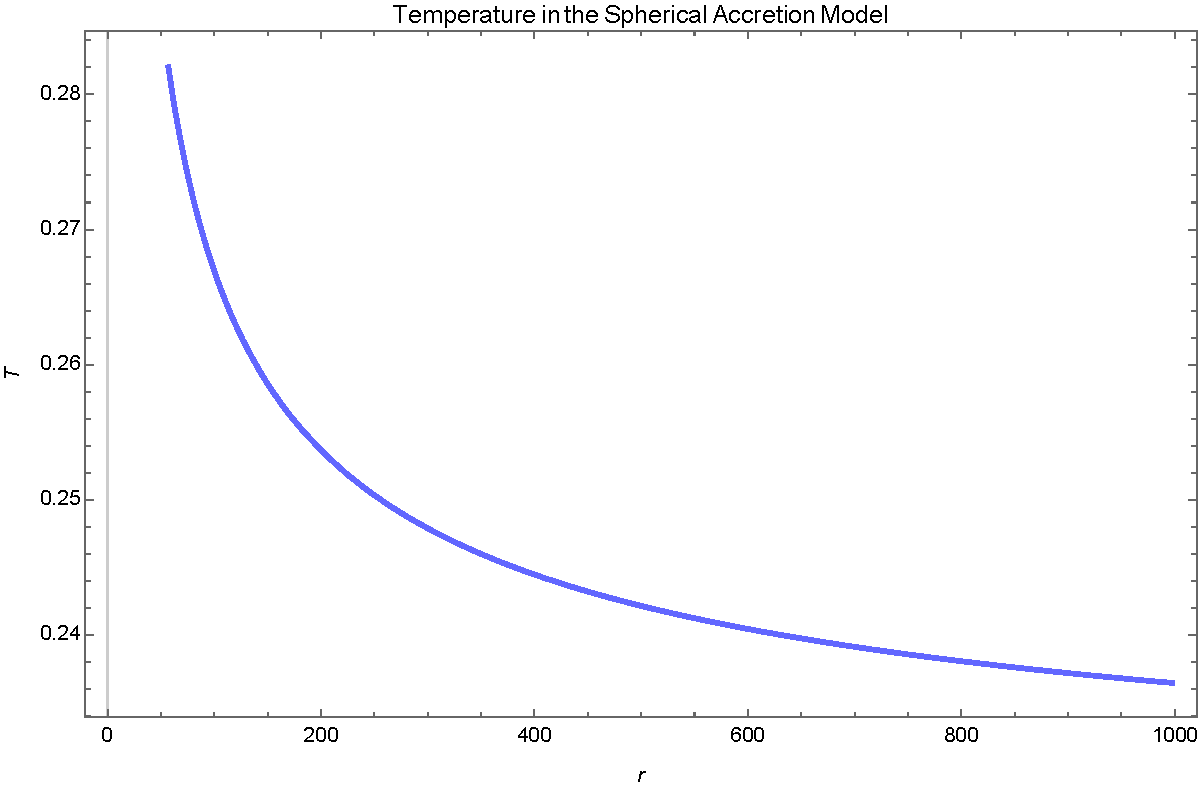
\includegraphics[scale=0.45] {figures/Temperature.pdf}
      \end{figure}
	\end{center}	
\end{frame}

\begin{darkframes}

\begin{frame}{Next Lecture}
  	\Large
	{09. Accretion Disks}
\end{frame}

  
\end{darkframes}
\end{document}
